	Here we analyze the behavior of the explicit Linear Steklov method (\SM) for scalar and vector SDEs. 
The tests confirm the convergence order 1/2 for stochastic differential systems with locally Lipschitz drift 
and suggest that the \SM scheme reproduces almost surely stability (a.s.). We validate the efficiency of the new 
method  by comparing with other actual methods like the Euler-Maruyama, Backward Euler (BEM) \cite{Mao2013} and tamed 
Euler (TEM) \cite{Hutzenthaler2012c}. All simulations are implemented in Python 2.7 and we use the Mersenne random 
number generator with fixed seed 100.

\subsection{Scalar SDE}	
	
{\textbf{Example 1.}} We examine the \SM method using a SDE with super-linear grow diffusion. We 
	consider the SDE reported by \citeauthor*{Tretyakov2013} in \cite[Eq. (5.6)]{Tretyakov2013}
	\begin{equation}\label{eqn:SDETretyakov}
		dy(t) =
		\left(
			1-y^5(t) +y^3(t)  
		\right) dt
		+
		y^2(t) dW(t), \qquad y_0=0.
	\end{equation}
	\citeauthor{Tretyakov2013} shows via simulation of \eqref{eqn:SDETretyakov} that the increment-tamed scheme
	\cite[Eq(1.5)]{Hutzenthaler2015}
	\begin{equation}\label{eqn:Increment-Tamed}
		X_{k+1} = X_k + 
			\frac{
				f(X_k) h + 
				g(X_k)\Delta W_k 
			}{
			\max\left(
				1, h
				\left|
					h f(X_k) +
					g(X_k)\Delta W_k
				\right|
			\right)}
	\end{equation}
	produces spurious oscillations. \citeauthor{Hutzenthaler2015} prove the convergence of this scheme under
	linear growth condition over diffusion. So, this suggest us that only certain kind of 
	explicit schemes with convergence under globally Lipschitz and linear growth diffusion conditions	
	%globally Lipschitz diffusion and linear growth 
	can extended their convergence to a locally Lipschitz diffusion and other kind of growth bound.
	Using $a(x):= -x^4 +x^2$, $b: = 1$ and $E=\{-1,0,1\}$, we construct the \SM method
	\begin{equation}\label{eqn:TreyakovLSMethod}
		Y_{k+1} = \exp(ha(Y_k))Y_k + 
		\frac{\exp(ha(Y_k)) - 1}{a(Y_k)} \1{E^c}
		+h\1{E}
		+Y_k^2\Delta W_k. 		
	\end{equation}
	\Cref{fig:Tretyakov} shows the numerical solution of SDE \eqref{eqn:SDETretyakov} with the Increment-Tamed (I-TEM) 
	\eqref{eqn:Increment-Tamed}, \SM method \eqref{eqn:TreyakovLSMethod}, and the Tamed (TEM) scheme with. 
	We consider the implicit Midpoint scheme \cite[Eq.(5.3)]{Tretyakov2013} with $h=\num{e-4}$ 	as reference.
	\begin{figure}[h!]
		\centering
		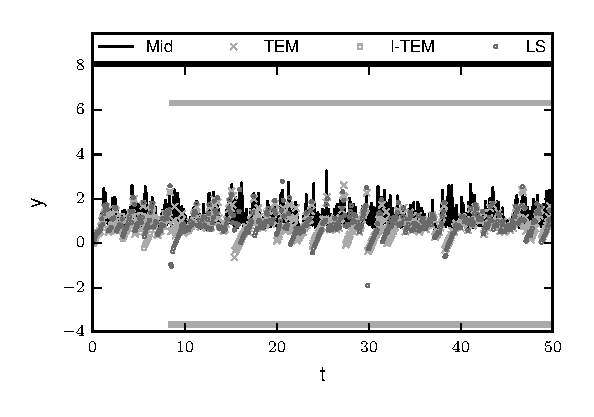
\includegraphics{Tretyakov}
		\caption{
			Numerical solution of SDE \eqref{eqn:SDETretyakov} using the I-TEM 
			\eqref{eqn:Increment-Tamed}, \SM method \eqref{eqn:TreyakovLSMethod}  and TEM
			with $h=\num{0.1}$, the reference solutions is a Midpoint rule approximation with $h=\num{e-4}$.
			}
		\label{fig:Tretyakov}
	\end{figure}
\subsection{Stochastic Differential Systems}
{\textbf{Example 1.}}
Now we compare the order of convergence
and the run time of the \SM method withthe TEM scheme as in \cite{Hutzenthaler2012a}. That is,
we consider a  Langevin equation under  the $d$-dimensional potential 
$U(x)= \frac{1}{4}|x|^4 - \frac{1}{2}|x|^2$, and $d$-dimensional Brownian additive noise. The corresponding
SDE reads
\begin{equation}\label{eqn:SDELangevinHutz}
dy(t) = 
\left(
y(t) - |y(t)| \cdot y(t)
\right)dt
+dW(t), \qquad y(0)=0.
\end{equation}
This model describes the motion of a Brownian particle of unit mass immersed on the potential $U(x)$. 
Taking $a_j(x):=1-|x|$ and $b_j=0$, $j\in 1\dots d$ we obtain the \SM method
\begin{equation}\label{eqn:LangevinLSMethod}
	Y_{k+1} = \diag
	\left[		
		e^{h a_1(Y_k)}, \dots, e^{ha_d(Y_k)}) 
	\right] 
	Y_k+
		\Delta W_k.
\end{equation}
\Cref{tbl:OrdersLS} shows the root means square errors at a final time $T=1$, which is approximated by
	\begin{equation}
		\sqrt{\EX{|Y_N - y(T)|^2}} \approx 
		\frac{1}{M}
		\left(
			\sum_{i=1}^M
			|y_i(T) - Y_{N,i}|^2	
		\right)^{1/2},
	\end{equation}
over a sample of $M$ =\num{10000} trajectories of the TEM, \SM  and BEM solutions to SDE \eqref{eqn:SDELangevinHutz} 
with dimension $d=10$.  We consider the TEM solution with step $h=2^{-19}$ as reference solution. 
In this experiment we confirm that the \SM method converges with standard order 1/2  and is almost equal accurate than 
the TEM.

	In some application as in Browninan Dynamics Simulations \cite{Cruz2012}, the dimension of a SDE
increases considerable the complexity and computational cost --- this prohibits the use of implicit methods.
\Cref{fig:TimeVsDimension} supports this (for SDE\eqref{eqn:SDELangevinHutz}): the runtime of BEM depends on 
dimension in a quadratic way, while the \SM and TEM depends on linear form.     
\begin{table}[t]
	\centering
	\begin{tabular}{lllllll}
		&        TEM &        	& LS		&           & BEM		 &         \\
		\toprule
		h		& ms-error	 & ECO 		& ms-error	    & ECO		& ms-error	 &	ECO	  \\
		\midrule
		$2^{-2}$	& \num{1.70388}    & ---		&\num{1.55394}		& ---		& \num{1.38157}	& 
		--- \\
		$2^{-3}$	& \num{1.16977}    & \num{0.54}     &\num{1.10775}    & \num{0.48} & \num{1.05309}	& 
		\num{0.39} \\ 
		$2^{-7}$	&\num{0.27895}     & \num{0.48} & \num{0.27795}   & \num{0.48} & \num{0.276895}& 
		\num{0.48} \\
			$2^{-11}$	& \num{0.07010}  & \num{0.50} & \num{0.07009}  & \num{0.50} & \num{0.07007} & 
		\num{0.50} \\
			$2^{-15}$	& \num{0.01739}  & \num{0.51} & \num{0.01739}  & \num{0.51} & \num{0.01739}& 
		\num{0.51} \\
		\num{0.00617}&\num{0.50} \\
		\bottomrule
	\end{tabular}
	\caption{
		Mean square errors and the experimental convergence order (ECO) for the SDE \eqref{eqn:SDELangevinHutz} with 
		a TEM with $h = 2^{-19}$ as reference solution.
	}\label{tbl:OrdersLS}
\end{table}
\begin{figure}[t]
	\centering
	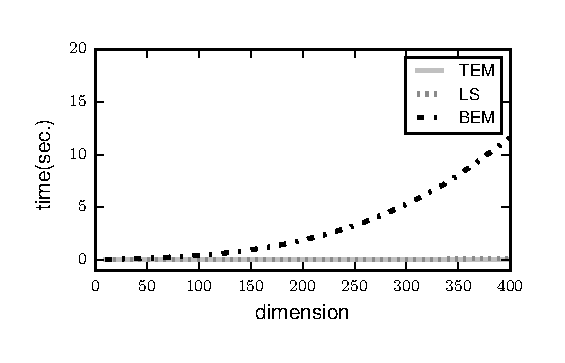
\includegraphics{TimeVsDimension}
	\caption{
		Runtime calculation of $Y_N$ with $h=2^{-17}$, using the BEM,  \SM and TEM methods for 
		SDE \eqref{eqn:SDELangevinHutz}.
	}
	\label{fig:TimeVsDimension}
\end{figure}

	
{\textbf{Example 2.}}
	\citeauthor{Hutzenthaler2012a} improve convergence of the Euler method by taming the drift increment term with 
	the factor
	$
	\frac{1}{1 + h |f(Y_k)|},
	$
	as consequence, the norm of  
	$
	\frac{h f(Y_k)}{1 + h |f(Y_k)|},
	$ is bounded by 1, which  controls the drift contribution of the TEM method at each step. This idea works very well
	over SDEs with drift contribution and initial condition that are comparable with this bound. However, we observed
	that on models where the	drift contribution has other scales, the TEM over damps the drift contribution. To fix
	ideas, we consider the	stochastic model reported in \cite{Dalal2008},
	\begin{align}\label{eqn:StochasticHIVDynamics}
	dy_1(t) &=
	\left(
	\lambda -\delta y_1(t) - (1 - \gamma) \beta y_1(t) y_3(t)
	\right)dt
	-\sigma_1 y_1(t) dW^{(1)}_t, 
	\notag \\
	dy_2(t) &= 
	\left(
	(1- \gamma) \beta y_1(t) y_3(t) - \alpha y_2(t) 
	\right)dt
	-\sigma_1 y_2(t) dW^{(1)}_t, 
	\\
	dy_3(t) & = 
	\left(
	(1 - \eta) N_0 \alpha y_2(t) 
	-\mu y_3(t)
	-(1 - \gamma ) \beta y_1(t) y_3(t) 
	\right)dt
	- \sigma_2 y_3(t) dW^{(2)}_t.
	\notag
	\end{align}	
	\begin{figure}[h!]
		\centering
		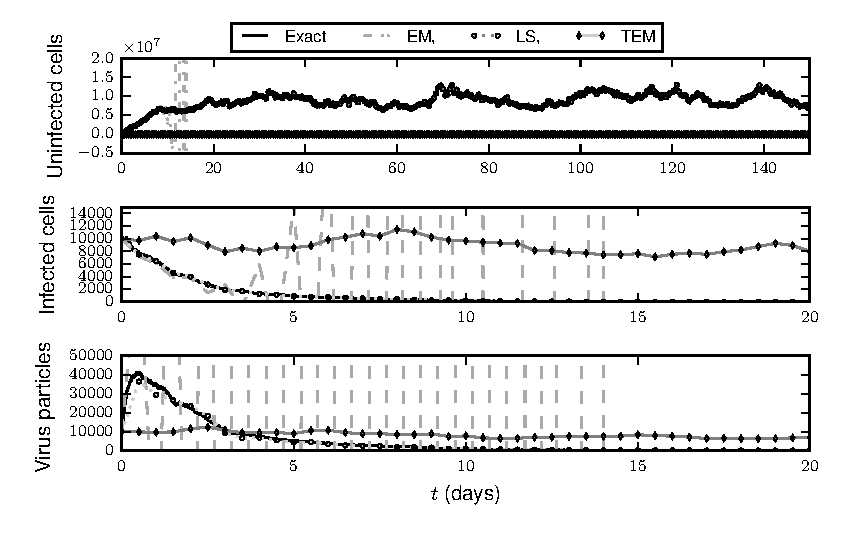
\includegraphics{./InternalHIVDynamics5e-1}
		\caption{
			Likening between EM, \SM, TEM approximations for SDE \eqref{eqn:StochasticHIVDynamics} with
			$\gamma = \num{0.5}$,
			$\eta = \num{0.5}$,
			$\lambda = \num{e6}$, 
			$\delta = \num{0.1}$,
			$\beta = \num{e-8}$,
			$\alpha = \num{0.5}$,
			$N_0= \num{100}$,
			$\mu = \num{5}$,
			$\sigma_1 = \num{0.1}$,
			$\sigma_2 = \num{0.1} $,
			$y_0 = (
				\num{10000},%{\per\cubic\deci\meter}, 
				\num{10000},%{\per\cubic\deci\meter}, 
				\num{10000}.%{\per\cubic\deci\meter}
			)^T$,
			$h=\num{0.5}$.
			Here the reference solution means a BEM simulation
			with the same parameters but with a step-size $h=\num{e-5}$.
		}
		\label{fig:InternalHIVDynamics5e-1}
	\end{figure} 
	Here we use the following \SM method. Taking 
	\begin{align*}
		E_1&:=	\left\{
			(x,y,z)^T \in \R^3:
			z=0 \text{ or }
			\frac{-\delta}{\beta(1-\gamma)}
		\right\}, \quad
		E_2:=	\emptyset, \quad   %\\
		E_3:=  \left\{ (x,y,z)^T \in \R^3: x=0 \right\},
	\end{align*}
	
	
	\begin{align}
		a_{1}(Y_k)) &:= 
			-\left(
				\delta + (1 - \gamma) \beta Y_k^{(3)}
			\right),		
			& b_1(Y_k^{(-1)}) &:= \lambda, 
			& 
		\notag
		\\
		a_{2}(Y_k) &:= -\alpha,
			&b_2(Y_k^{(-2)}) & :=
			(1-\gamma) \beta Y_{k}^{(1)} Y_{k}^{(3)},
		\notag
		\\
		a_{3}(Y_k) &= 
		-
		\left(
			\mu + (1- \gamma) \beta Y_{k}^{(1)}
		\right),
		\qquad
	%
		&b_{3}(Y_k^{(-3)}) &:= 
		\left(
			1 - \eta 
		\right)
		N_0 \alpha Y_{k}^{(2)},
		\notag			
	\end{align}
	 the \SM method for the stochastic model \eqref{eqn:StochasticHIVDynamics} reads,
	\begin{align}
		Y_{k+1} &= A^{(1)}(h,Y_k) \,Y_k + A^{(2)}(h,Y_k)b(Y_k)+ g(Y_k)\, \Delta W_k,
		\qquad \Delta W_k = \left(W_k^{(1)}, W_k^{(2)}\right)^T, 
		\notag\\ 
		A^{(1)}(h,Y_k)&:=
		\begin{pmatrix}
		e^{ha_1(Y_k)}	&	0	&0 \\
		0	&e^{ha_2(Y_k))}	&0\\
		0	&0				&e^{ha_3(Y_k))}
	\end{pmatrix},
%	
	\notag
	\\
	%	
	A^{(2)}&:=
	\begin{pmatrix}
		h \Phi_1(Y_k)\1{E_1^c}	&0	&0\\
		0 & 
			\left(\displaystyle
					\frac{e^{-h\alpha} - 1}{\alpha}
			\right) & 0\\
		0 & 0 & h \Phi_3(Y_k)\1{E_3^c} 
	\end{pmatrix}
	%\notag \\
	+h
	\begin{pmatrix}
		\1{E_1}	&0 			&0\\
		0		&0			&0\\
		0		&0			&\1{E_3}\\
	\end{pmatrix},
	\notag
	\\
	b(Y_k) &:=
	\begin{pmatrix}
		b_1(Y_k^{(-1)})\\
		b_2(Y_k^{(-2)})\\
		b_3(Y_k^{(-3)})
	\end{pmatrix},
	\qquad
	g(Y_k):=
	\begin{pmatrix}
		-\sigma_1 Y_k^{(1)}	&0\\
		-\sigma_1 Y_k^{(2)}	&0\\
		0	&-\sigma_2 Y_k^{(3)}
	\end{pmatrix}.
\end{align}
	
\citeauthor{Dalal2008} in \cite[Thm 5.1]{Dalal2008} gives conditions over the parameter of SDE 
\eqref{eqn:StochasticHIVDynamics}, which assure a.s. exponential stability --- in the sense that
the infected cells ($y_2$) and virus particles ($y_3$) will tend to their equilibrium value 0 exponentially with 
probability 1---and verify this asymptotic behavior by
simulation 
%SDE \eqref{eqn:StochasticHIVDynamics} 
with parameters reported in published literature \cite{Bonhoeffer1997, Callaway2002, Nelson2000, Nowak1997}.
\Cref{fig:InternalHIVDynamics5e-1} shows a simulation path with same parameters with the \SM and TEM approximations.
We observe how the TEM oscillates around of initial condition while the \SM reproduce the underlying asymptotic
behavior.  
